\documentclass[conference]{IEEEtran}
\IEEEoverridecommandlockouts
% The preceding line is only needed to identify funding in the first footnote. If that is unneeded, please comment it out.
\usepackage{cite}
\usepackage{url}
\usepackage{amsmath,amssymb,amsfonts}
\usepackage{algorithmic}
\usepackage{graphicx}
\usepackage{textcomp}
\usepackage{xcolor}
\def\BibTeX{{\rm B\kern-.05em{\sc i\kern-.025em b}\kern-.08em
    T\kern-.1667em\lower.7ex\hbox{E}\kern-.125emX}}
\begin{document}
\bibliographystyle{IEEEtran}
\title{
\includegraphics[width=5cm]{images/ust.png}\linebreak DreamHarmony: Unveiling Sleep Patterns through Lifestyle Modeling and Predictive Analytics
}


\author{\IEEEauthorblockN{Hoang Q. Nguyen\IEEEauthorrefmark{1}\IEEEauthorrefmark{3}, Md Mahmudul Hassan\IEEEauthorrefmark{1}\IEEEauthorrefmark{3}, Solomon Rukundo\IEEEauthorrefmark{2}\IEEEauthorrefmark{3}}
    \IEEEauthorblockA{\IEEEauthorrefmark{1} Korea Institute of Science and Technology}
    \IEEEauthorblockA{\IEEEauthorrefmark{2} Korea Research Institute of Standards and Science}
    \IEEEauthorblockA{\IEEEauthorrefmark{3} Korea National University of Science and Technology (UST)}
}
\maketitle

\begin{abstract}
    This study investigates how daily habits like exercise and technology use are related to sleep quality. After careful data preparation, we used statistical methods, including Pearson\cite{pearson} and Spearman correlations\cite{spearman}, to identify which lifestyle factors are most connected to good or poor sleep, in terms of duration and quality. We then built various mathematical models, such as linear regression and decision trees, to predict sleep quality based on these factors. Our results show that some daily activities have a strong link to how well people sleep, and our models can explain a significant part of this link. These findings could help guide recommendations for improving sleep based on personal habits.
\end{abstract}

\begin{IEEEkeywords}
    big data, sleep, health, lifestyle, machine learning, support vector machine
\end{IEEEkeywords}

\section{Introduction}
The interplay between lifestyle and sleep quality is an increasingly pertinent subject in the realm of public health. To explore this intricate relationship, we embarked on a comprehensive data collection campaign, developing a structured survey that captures a wide array of lifestyle variables alongside sleep metrics. The survey's design allowed for the nuanced capture of daily routines, technological interactions, and exercise habits.

Post-collection, data processing commenced with rigorous cleaning techniques to ensure integrity and analytical viability. Our initial exploratory analysis hinged on the construction of a correlation matrix heatmap, which served as a visual aid to discern potential relationships between variables. This graphical representation provided the preliminary clues necessary for subsequent hypothesis formulation.

Armed with hypotheses, we delved into a variety of statistical tests. Spearman's rank correlation offered insights into monotonic relationships, while Pearson's correlation assessed linear dependencies. For categorical data, the Chi-squared test\cite{chi} evaluated associations between discrete variables. These statistical methodologies were pivotal in distilling the factors most relevant to sleep quality.

The culmination of our hypothesis testing informed the selection of variables for model fitting. We implemented a variety of machine learning models, including, but not limited to, regression analyses, decision trees, and support vector machines. Each model was rigorously evaluated to determine its predictive power and relevance to our study.

Our contributions through this research are multifaceted. Initially, we developed a foundational survey engineered to assess sleep and lifestyle variables. Subsequently, we discerned pivotal factors that influence sleep quality by leveraging statistical analysis and hypothesis testing. Furthermore, we harnessed machine learning algorithms to construct models based on these factors. Our study establishes a framework for future exploration, highlighting the necessity for continuous data accumulation to refine and augment model efficacy. We invite researchers and the public alike to contribute to our ongoing work (available on GitHub\footnotemark) through feedback and new applications of our findings.
\footnotetext{\url{https://github.com/johnkimtech/sleep}}



\section{Related Work}
A large Japanese cross-sectional study (n = 30,000) found that 28\% slept less than 6 hours per night and 65\% slept less than 7 hours per night despite 80\% claiming adequate sleep \cite{lifestyleinfluence}. Logistic regression identified short sleep duration (\textless 6 hours) as associated with being female, younger age, urban living, unemployment, poor health, lack of exercise, and irregular eating \cite{lifestyleinfluence}. A review of Asian literature linked insufficient sleep to high stress, high BMI/obesity, and depression \cite{immune}. A study of Lithuanian university students (n = 405) found poor sleep quality, especially among medical students, to be associated with high academic demands, anxiety, limited leisure time, and academic dissatisfaction \cite{lithua}. These findings suggest that interventions targeting stress, leisure time, exercise, urban planning, mental health, and other lifestyle factors could potentially improve sleep \cite{lifestyleinfluence,lithua}. However, existing research lacks exploration of newer lifestyle factors, such as the impact of technology and social media on sleep habits. Future research is needed to investigate how emerging habits like nighttime electronic device use, pre-sleep social media engagement, and internet overuse might contribute to sleep disturbances.

\section{Data Acquition \& Preprocessing}
The DreamHarmony Sleep Survey was an integral part of our study, designed to explore the multifaceted relationship between lifestyle habits and sleep quality. To capture a diverse set of responses, the survey was made available in multiple languages including Korean, English, Vietnamese, and Bengali.

\subsection{Data collection through online survey}
The DreamHarmony Sleep Survey was meticulously designed to delve into the myriad factors affecting sleep quality and patterns. This comprehensive survey aimed to unravel the complex interplay between lifestyle habits and sleep, potentially leading to enhancements in sleep quality and overall life satisfaction.
\subsubsection*{Survey Structure and Distribution}

The survey was structured into distinct sections: demographics, lifestyle, and sleep habits. It was distributed via Google Forms\cite{dhsurvey} through the authors' social networks, encompassing friends, colleagues, and family members. While this method facilitated rapid data collection, we acknowledge the potential for bias and sample imbalance due to the nature of the distribution channels.

\subsubsection*{Demographics}

Participants were queried about their age, gender, education level, and occupation. This demographic information was crucial to understanding the contextual background of each respondent.

\subsubsection*{Lifestyle and Sleep Habits}

The lifestyle section encompassed questions regarding exercise frequency, device usage, and screen time before sleep. In the sleep habits section, we focused on gathering detailed information about participants' sleep patterns. Key questions included:
\begin{itemize}
    \item\textbf{Bedtime and Wake-up Time}: These questions helped calculate the actual duration of nighttime sleep, a vital metric for assessing sleep quality.
    \item\textbf{Sleep Quality}: Respondents rated their overall sleep quality, providing us with a subjective assessment of their sleep experience.
    \item\textbf{Sleep Onset}: We inquired about the time it typically takes for respondents to fall asleep, aiming to understand sleep onset difficulties.
    \item\textbf{Sleep Medication}: This question ascertained whether participants use any medication to aid their sleep, which is indicative of sleep quality issues.
    \item\textbf{Sleep Disturbances}: The frequency of disturbances such as waking up during the night or experiencing restless sleep was also captured.
\end{itemize}
\subsubsection*{Contributions}
Our survey, though limited by its distribution method, provides valuable insights into sleep quality and its influencing factors. The subsequent statistical and machine learning analyses contribute to a nuanced understanding of sleep dynamics, laying the groundwork for future research in this field.
\subsection{Preprocessing: Translation, Merging, and Cleanup}
\subsubsection*{Translation}
To harness the collected data effectively in the subsequent stages of analysis, it was imperative to amalgamate the survey responses from all language versions into a single dataframe. This posed significant challenges, as the survey questions and responses were presented in various languages, and even the English version contained verbose questions and answers. To address these issues, we:

\begin{enumerate}
  \item Constructed a JSON file containing a translation mapping from the original column headers to abbreviated column headers in English.
  \item Utilized the \texttt{rename} function from the \texttt{pandas} library to update the dataframe with the new headers \cite{dfrename}.
\end{enumerate}

For the translation of cell values, a similar approach was employed, where JSON files served as the translation mapping. These mappings were then applied to the dataframe using the \texttt{map} function to convert the cell values into concise English terms \cite{dfmap}.

\subsubsection*{Merging \& Cleanup}
Once translations for both headers and cell values were standardized, we employed the \texttt{concat} function from \texttt{pandas} to stack the individual dataframes from each language version into a unified dataframe \cite{pdconcat}. However, this merged dataset contained several inconsistencies, including:

\begin{itemize}
  \item Heights recorded as less than 100cm, primarily in the Bengali version of the survey, where respondents preferred inches to centimeters. For these cases, heights were converted from inches to centimeters.
  \item Respondents' confusion between 24-hour and 12-hour time formats, resulting in miscalculations of sleep duration, with some reported durations nearing 20 hours per day. We addressed this by filtering out erroneous values and correcting the time format.
\end{itemize}
Furthermore, actual night sleep duration was calculated from the 'Bedtime' and 'Wake-up Time' responses. For respondents providing height and weight, Body Mass Index (BMI) was computed, offering additional metrics pivotal to the analysis. Following these corrections, the dataset was ready for subsequent stages of examination.
\section{Analysis}
\subsubsection*{Descriptive statistics}
\begin{table}[htbp]
    \centering
    \caption{Descriptive statistics of the sleep study data}
    \label{tab:sleep_data1}
    \begin{tabular}{lrrrrr}
    \hline
    & Height (cm) & Weight (kg) & BMI & Sleep Quality & Night Sleep\footnotemark \\ \hline
    count & 83 & 92 & 80 & 108 & 105 \\
    mean & 165.31 & 67.42 & 24.55 & 3.44 & 7.04 \\
    std & 8.32 & 12.80 & 4.25 & 0.82 & 1.37 \\
    min & 150.00 & 43.00 & 18.52 & 2.00 & 1.67 \\ \hline
    25\% & 160.00 & 59.80 & 22.02 & 3.00 & 6.50 \\
    50\% & 167.00 & 68.00 & 24.69 & 3.00 & 7.00 \\
    75\% & 171.00 & 75.00 & 27.31 & 4.00 & 8.00 \\
    max & 185.00 & 100.00 & 35.85 & 5.00 & 9.75 \\
    \hline
    \end{tabular}
\end{table}
\footnotetext{Calculated night time sleep based on Bedtime and Wake-up time}

\begin{table*}
    \centering
    \caption{Descriptive statistics of sleep study participants}
    \label{tab:sleep_data2}
    \begin{tabular}{lrrrrr}
    \hline
    & Age Group & Gender & Education Level & Occupation & Exercise (days/week) \\ \hline
    count & 108 & 108 & 108 & 108 & 108 \\
    unique & 5 & 3 & 4 & 7 & 4 \\
    top & 25-34 & Male & Master's & Student & 1-2 Days \\
    freq & 72 & 67 & 47 & 47 & 43 \\ \hline
    & Device Usage (hrs/day) & Screen Time Before Sleep (hrs/min) & Sleep Onset (min) & Bedtime & Wake-up Time \\ \hline
    count & 108 & 108 & 108 & 104 & 108 \\
    unique & 4 & 4 & 4 & 18 & 20 \\
    top & 7+ Hours & 30-60mins & 15-30mins & 23:00 & 07:00 \\
    freq & 43 & 45 & 55 & 24 & 18 \\ \hline

    & Nap Duration (min) & Sleep Duration (hrs/24hr) & Sleep Disturbances & Sleep Medication & Language \\ \hline
    count & 108 & 107 & 108 & 108 & 108 \\
    unique & 5 & 3 & 5 & 2 & 4 \\
    top & No Nap & 6hrs+ & Rarely & No & English \\
    freq & 61 & 64 & 48 & 48 & 68 \\ \hline

    \end{tabular}
    \end{table*}
    

As shown in Table~\ref{tab:sleep_data1} and \ref{tab:sleep_data2}:
\begin{itemize}
    \item \textbf{Sleep quality}: Respondents rated their sleep quality around 3 on a 5-point scale, indicating moderate quality.
    \item \textbf{BMI}: The average Body Mass Index (BMI) is around 23.55, ranging from 16.5 to 39.4.
    \item \textbf{Night sleep duration}: The average night sleep duration is around 7 hours, with a wide range of 1.67 to 9.75 hours.\item \textbf{Age Group}: The most common age group among respondents is 25-34.
    \item \textbf{Gender}: A slightly higher number of male respondents compared to females.
    \item \textbf{Education Level}: The majority of respondents have a Master's degree.
    \item \textbf{Occupation}: Many respondents are students.
    \item \textbf{Exercise Days/Week}: '1-2 Days' is the most common response for exercise frequency.
    \item \textbf{Device Usage (hrs/day)}: A large portion of respondents use devices for '7+ Hours' per day.
    \item \textbf{Screen Time Before Sleep}: '30-60 Minutes' is the most common duration for screen time before sleep.
    \item \textbf{Sleep Disturbances}: 'Rarely' is the most frequent response, indicating that most respondents rarely experience sleep disturbances.
    \item \textbf{Sleep Medication}: The majority of respondents do not use sleep medication.
    \item \textbf{Language}: English is the most common language among respondents.

\end{itemize}  

\subsubsection*{Distribution Analysis}
The analysis of sleep quality and night sleep duration distributions, as depicted in Figures \ref{fig:distsleep} and \ref{fig:distsleepwm}, reveals the following insights:

\begin{itemize}
    \item \textbf{Sleep Quality Distribution:} 
    The majority of the respondents report their sleep quality within the range of 2 to 4, with a concentration of responses at a sleep quality score of 3. Notably, a smaller proportion of participants indicate experiencing excellent sleep quality, as reflected by the fewer scores of 5.

    \item \textbf{Night Sleep Duration Distribution:}
    Observations from the histogram suggest a normal distribution of sleep duration, predominantly centered around the 7-hour mark. This finding is in line with standard sleep recommendations. Notably, the occurrences of extremely short (\textless 5 hours) or long (\textgreater 9 hours) sleep durations are relatively infrequent.

    \item \textbf{Gender-Based Sleep Differences:} 
    The boxplots in Figure \ref{fig:distsleepwm} indicate a striking similarity in sleep quality between male and female participants. Additionally, the comparison of night sleep duration across genders reveals closely aligned distributions, with minor variations primarily in the lower and upper quartiles.
\end{itemize}

These observations contribute to a nuanced understanding of the distribution patterns of sleep quality and duration among the survey participants, highlighting subtle differences and commonalities in sleep experiences.

\begin{figure}[ht]
    \centering
    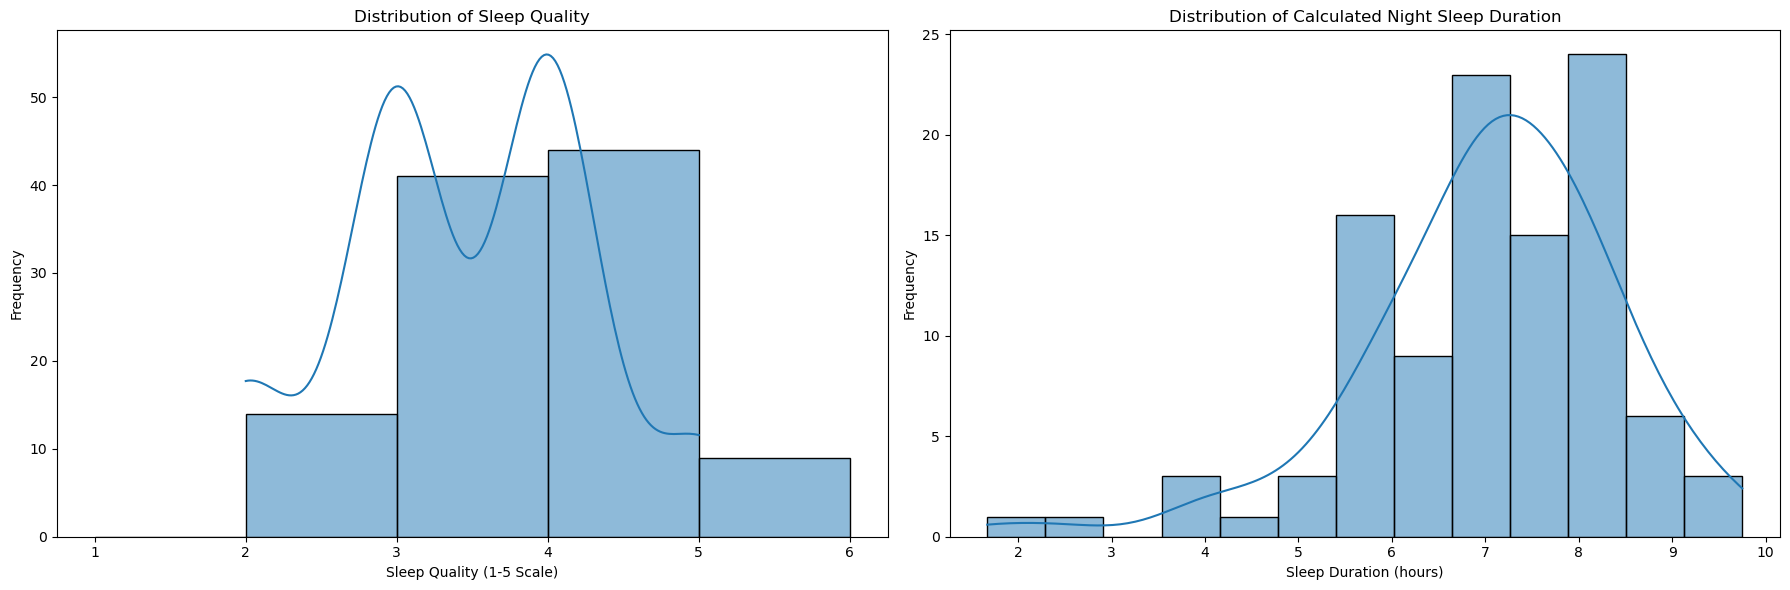
\includegraphics[width=8cm]{images/distsleep.png}
    \caption{Distribution of Sleep Quality and Duration}
    \label{fig:distsleep}
  \end{figure}
  \begin{figure}[ht]
      \centering
      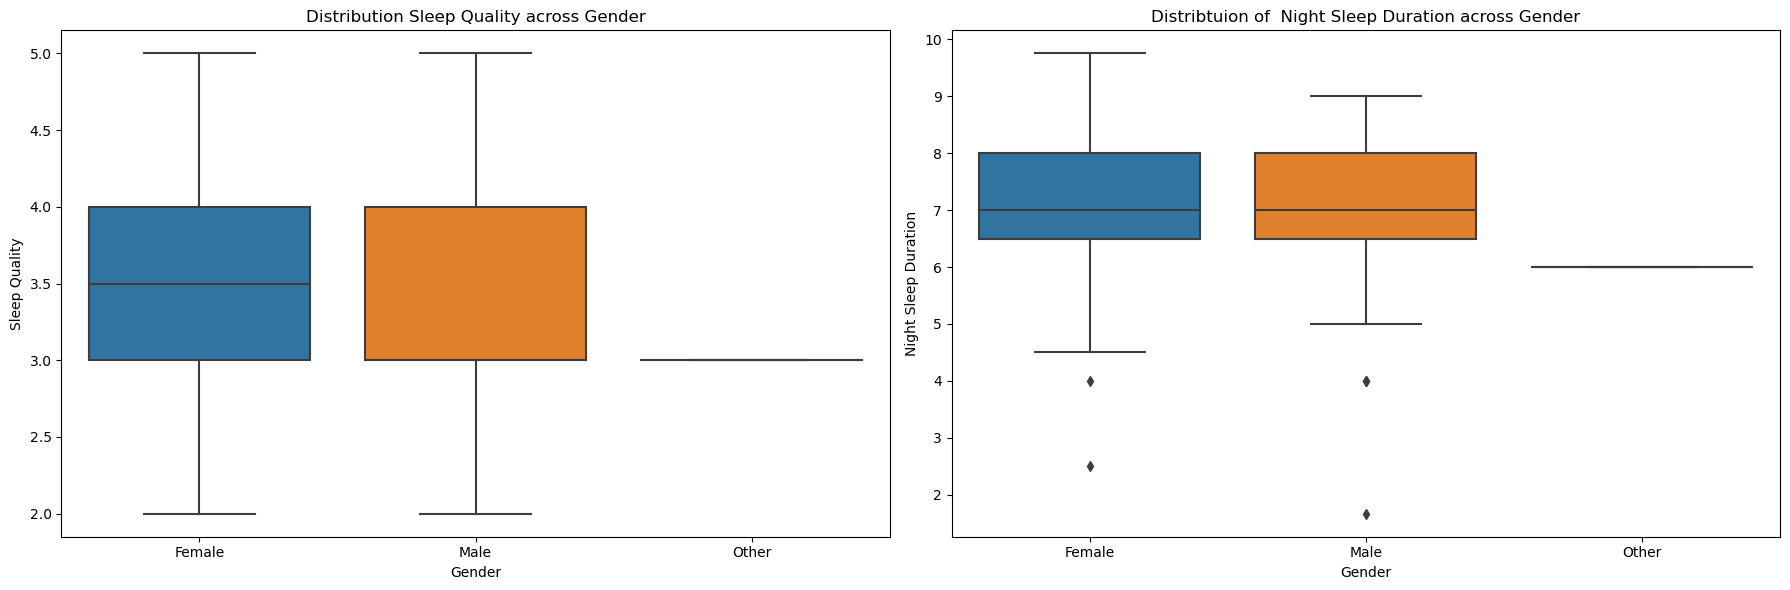
\includegraphics[width=8cm]{images/distsleepwm.png}
      \caption{Distribution of Sleep Quality and Duration across Gender}
      \label{fig:distsleepwm}
    \end{figure}


    \subsubsection*{Correlation analysis}
    The heatmap in Figure \ref{fig:corrheat} illustrates these following correlations:
    \begin{itemize}
        
\item \textbf{Sleep Quality:} Strong negative correlation with Sleep Disturbances (-0.55), indicating better sleep quality is associated with fewer disturbances.
Moderate negative correlation with Sleep Onset Time (-0.32), suggesting that quicker sleep onset is associated with better sleep quality.

\item \textbf{BMI:} Slight negative correlation with Calculated Night Sleep Duration (-0.19), suggesting that higher BMI might be slightly associated with shorter sleep duration, although the relationship is weak.
Moderate negative correlation with Device Usage (-0.28), indicating that higher BMI is associated with less device usage.

\item \textbf{Calculated Night Sleep Duration:} Negative correlation with Age Group (-0.23), indicating that older age groups might have shorter sleep duration.
All other correlations with Calculated Night Sleep Duration are weak.

\item \textbf{Age Group:} Moderate positive correlation with BMI (0.31), suggesting that higher BMI values are more prevalent in older age groups.

\item \textbf{Sleep Onset Time:} No significant correlations with other variables, aside from the moderate negative correlation with Sleep Quality.

\item \textbf{Nap Duration:} Weak correlations with all other variables.

\item \textbf{Exercise Days/Week:} Slight positive correlation with Calculated Night Sleep Duration (0.22), implying that more exercise might be related to slightly longer sleep duration.
Weak correlations with all other variables.

\item \textbf{Sleep Disturbances:} Aside from the strong negative correlation with Sleep Quality, Sleep Disturbances show weak correlations with other variables.

\item \textbf{Device Usage (hrs/day):} Moderate negative correlation with BMI (-0.28), as previously mentioned.
Weak correlations with all other variables.
This heatmap indicates that while some variables are correlated, most relationships are weak. The strongest observed relationships involve sleep quality, particularly its negative correlation with sleep disturbances and sleep onset time. This suggests that variables affecting the quality of sleep have a more significant impact on sleep disturbances and the time it takes to fall asleep. The correlations involving BMI, age group, and device usage suggest demographic and behavioral patterns but are not strong enough to imply causation.
    \end{itemize}
    \begin{figure}[ht]
        \centering
        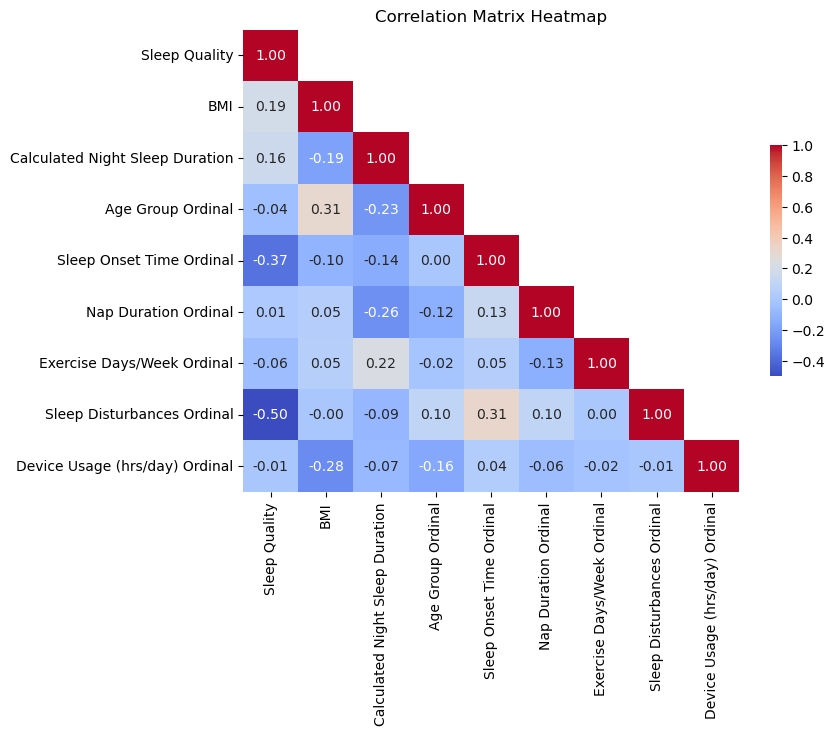
\includegraphics[width=8cm]{images/corrheat.png}
        \caption{Correlation Heatmap between variables}
        \label{fig:corrheat}
      \end{figure}
\section{Hypothesis Testing}
\subsection*{Overview}

The observed correlations from the data analysis and visualizations suggest several hypotheses that could be explored through further analysis:
      \begin{itemize}

        \item \textit{Impact of Sleep Disturbances on Quality:} Given the strong negative correlation between sleep disturbances and quality, we can hypothesize that increased sleep disturbances are likely to negatively impact the quality of sleep.

        \item \textit{Age in Relation to Sleep Duration:} The negative correlation between age and calculated night sleep duration leads to the hypothesis that sleep duration may decrease with age.
        
        \item \textit{Relationship Between Sleep Onset Time and Quality:} The moderate negative correlation observed between sleep onset time and quality suggests that a longer time to fall asleep might be associated with poorer sleep quality.
        
        \item \textit{Influence of Exercise on Sleep Duration and Quality:} The slight positive correlation between exercise days per week and sleep duration hints at a potential hypothesis that increased physical activity could contribute to longer and possibly better quality sleep.
        
        \item \textit{Nap Duration's Effect on Nighttime Sleep Duration:} Although the correlation is weak, we could investigate whether the duration of naps has any effect on the duration of nighttime sleep.
      \end{itemize}
      \subsection*{Hypothesis I - Increased Sleep Disturbances Negatively Impact Sleep Quality}
      \textit{Null Hypothesis (\(H_0\))}: The level of Sleep Disturbances has no impact on Sleep Quality.
      
      \textit{Alternative Hypothesis (\(H_1\))}: The level of Sleep Disturbances negatively impacts Sleep Quality.
      
      To investigate the relationship between sleep disturbances and sleep quality, we utilized Spearman's rank correlation due to its ability to measure monotonic relationships without assuming a linear relationship between variables, which is suitable for ordinal data. Additionally, the Chi-squared test was employed to evaluate the independence of categorical variables.
      
      \begin{table}[ht]
      \centering
      \caption{Statistical Tests for Sleep Disturbances and Sleep Quality}
      \label{tab:hypothesis1}
      \begin{tabular}{|c|c|c|c|}
      \hline
      \textbf{Test Type} & \textbf{Statistic} & \textbf{P-value} & \textbf{Conclusion} \\
      \hline
      Spearman's \(\rho\) & -0.453 & \(4.2 \times 10^{-7}\) & Reject \(H_0\), accept \(H_1\)
      \\
      \hline
      Chi-squared & 46.03 & \(6.85 \times 10^{-6}\) & Reject \(H_0\), accept \(H_1\)
      \\
      \hline
      \end{tabular}
      \end{table}
      
      The Spearman correlation coefficient of -0.453 suggests a moderate negative correlation, indicating that increases in sleep disturbances are associated with decreases in sleep quality. Given the p-value of \(4.2 \times 10^{-7}\), which is substantially below the alpha threshold of 0.05, we reject the null hypothesis, affirming the alternative hypothesis of a negative impact of sleep disturbances on sleep quality.
      
      Similarly, the Chi-squared test yields a statistic of 46.03, surpassing the critical value for 12 degrees of freedom. Alongside a p-value of \(6.85 \times 10^{-6}\), this provides strong evidence against the null hypothesis, suggesting a significant association between sleep disturbances and sleep quality in our dataset.
      \subsection*{Hypothesis II - Older People Have Shorter Night Sleep}
\textit{Null Hypothesis (\(H_0\))}: Age group has no impact on Sleep Duration.

\textit{Alternative Hypothesis (\(H_1\))}: Age group has a negative correlation with Sleep Duration.\\
The Pearson test was chosen for its ability to detect linear relationships between two continuous variables. Given the fairly normal distribution of Sleep Quality, it serves as an appropriate measure for this analysis. On the other hand, The Kendall’s Tau test was selected for its robustness in assessing the strength of association between two ordinal variables, making it suitable for the nature of our age group data.


\subsubsection*{Pearson Correlations Test}
The Pearson correlation coefficient was calculated as -0.232 with a p-value of 0.0088, indicating a weak negative correlation between age group and sleep duration. This suggests a trend where sleep duration may decrease slightly as age increases. Given the significance level of 0.05, the null hypothesis can be rejected in favor of the alternative.

\subsubsection*{Kendall’s Tau Test}
A Kendall’s Tau test yielded a correlation of -0.204 with a p-value of 0.00619, reinforcing the presence of a weak negative correlation. The results allow us to reject the null hypothesis, affirming the alternative that there is a statistically significant, though mild, negative association between age group and sleep duration.

\begin{table}[ht]
\centering
\caption{Statistical Tests for Age Group and Sleep Duration}
\label{tab:hypothesis2}
\begin{tabular}{|c|c|c|c|}
\hline
\textbf{Test Type} & \textbf{Correlation} & \textbf{P-value} & \textbf{Conclusion} \\
\hline
Pearson & -0.232 & 0.0088 & Reject \(H_0\), accept \(H_1\) \\
\hline
Kendall’s Tau & -0.204 & 0.00619 & Reject \(H_0\), accept \(H_1\) \\
\hline
\end{tabular}
\end{table}

Both tests corroborate the alternative hypothesis, suggesting that as individuals progress into higher age categories, a decrease in sleep duration may occur. However, the correlation is not strong, pointing to the influence of other factors not accounted for in this analysis.


\subsection*{Hypothesis III - Longer Sleep Onset Time Worsens Sleep Quality}
\textit{Null Hypothesis (\(H_0\))}: Increase in Sleep Onset Time has no impact on Sleep Quality.

\textit{Alternative Hypothesis (\(H_1\))}: Increase in Sleep Onset Time leads to a decline in Sleep Quality.

The relationship between Sleep Onset Time and Sleep Quality was analyzed using Spearman's rank correlation for its suitability with ordinal data and the Chi-squared test to assess variable independence.

\begin{table}[ht]
\centering
\caption{Statistical Testing of Sleep Onset Time Worsens Sleep Quality}
\label{tab:hypothesis3}
\begin{tabular}{|c|c|c|c|}
\hline
\textbf{Test Type} & \textbf{Statistic} & \textbf{P-value} & \textbf{Conclusion} \\
\hline
Spearman's \(\rho\) & -0.377641 & \(2.80 \times 10^{-5}\) & Reject \(H_0\), accept \(H_1\) \\
\hline
Chi-squared & 19.297 (DoF: 9) & 0.022782 & Reject \(H_0\), accept \(H_1\) \\
\hline
\end{tabular}
\end{table}

The Spearman correlation coefficient of -0.377641 suggests a moderate inverse relationship, where longer Sleep Onset Time is associated with poorer Sleep Quality. The p-value of \(2.80 \times 10^{-5}\) indicates that this correlation is statistically significant and not due to chance.

Similarly, the Chi-squared test with a statistic of 19.297119 and a p-value of 0.022782 also suggests a significant association between Sleep Onset Time and Sleep Quality. Though not a strong relationship, it is sufficient to reject \(H_0\) and accept \(H_1\), indicating a notable connection that warrants further investigation.


\subsection*{Hypothesis IVa - Weekly Exercise Frequency Improves Sleep Quality}
\textit{Null Hypothesis (\(H_0\))}: Weekly exercise frequency has no impact on Sleep Quality.

\textit{Alternative Hypothesis (\(H_1\))}: Weekly exercise frequency improves Sleep Quality.

Spearman's correlation was used to test for a potential positive association between exercise frequency and sleep quality.

\begin{table}[ht]
    \centering
    \caption{Spearman Correlation and Chi-squared Test for Exercise Frequency and Sleep Quality}
    \label{tab:hypothesis4a}
    \begin{tabular}{|c|c|c|c|}
    \hline
    \textbf{Test Type} & \textbf{Statistic} & \textbf{P-value} & \textbf{Conclusion} \\
    \hline
    Spearman's \(\rho\) & -0.0577 & 0.7235 & Accept \(H_0\), reject \(H_1\) \\
    \hline
    Chi-squared & 13.2199 & 0.1529 & Accept \(H_0\), reject \(H_1\) \\
    \hline
    \end{tabular}
    \end{table}

The Spearman test resulted in a correlation coefficient of -0.0577 with a p-value of 0.7235, indicating no meaningful relationship between exercise frequency and sleep quality. The negative coefficient suggests a slight inverse trend, but the high p-value shows this is likely due to chance.

The Chi-squared test further supports the lack of evidence for an association. With a Chi2 Stat of 13.2199 and a p-value of 0.1529, the result does not exceed the critical value required to reject the null hypothesis at the 0.05 significance level.

\textbf{Conclusion:}The data does not support a significant relationship between weekly exercise frequency and sleep quality. Both Spearman's correlation and the Chi-squared test outcomes suggest that other unexplored factors might be more influential in determining sleep quality.

\subsection*{Hypothesis IVb - Weekly Exercise Frequency Improves Sleep Duration}
\textit{Null Hypothesis (\(H_0\))}: Weekly exercise frequency has no impact on Sleep Duration.

\textit{Alternative Hypothesis (\(H_1\))}: Weekly exercise frequency improves Sleep Duration.

Spearman's correlation and ANOVA tests were conducted to evaluate the relationship between exercise frequency and sleep duration.

\begin{table}[ht]
\centering
\caption{Statistical Tests for Exercise Frequency and Sleep Duration}
\label{tab:hypothesis4b}
\begin{tabular}{|c|c|c|}
\hline
\textbf{Test Type} & \textbf{Statistic} & \textbf{P-value} \\
\hline
Spearman's \(\rho\) & 0.1805 & 0.0327 \\
\hline
ANOVA & 2.9423 & 0.0367 \\
\hline
\end{tabular}
\end{table}

The Spearman correlation coefficient of 0.1805 indicates a positive but weak relationship between exercise frequency and sleep duration, with a p-value of 0.0327 suggesting statistical significance.

The ANOVA test yields an F-statistic of 2.9423 and a p-value of 0.0367, confirming significant differences in sleep duration among different levels of exercise frequency.

\textbf{Conclusion:}
While the Spearman test suggests a positive correlation between exercise frequency and sleep duration, the relationship is weak. The ANOVA test reveals significant differences in sleep duration across exercise frequency groups. These findings imply that while an increase in exercise frequency might be associated with longer sleep duration, further analysis is required to fully understand the dynamics of this relationship.

\subsection*{Hypothesis V - Increased Nap Time Decreases Night Sleep Duration}
\textit{Null Hypothesis (\(H_0\))}: Increase in Nap Time has no impact on Night Sleep Duration.

\textit{Alternative Hypothesis (\(H_1\))}: Increase in Nap Time shortens Night Sleep Duration.

Spearman's correlation and Kendall’s Tau tests were conducted to assess the relationship between nap duration and night sleep duration.

\begin{table}[ht]
\centering
\caption{Statistical Tests for Nap Duration and Night Sleep Duration}
\label{tab:hypothesis5}
\begin{tabular}{|c|c|c|c|}
\hline
\textbf{Test Type} & \textbf{Statistic} & \textbf{P-value} & \textbf{Conclusion} \\
\hline
Spearman's \(\rho\) & -0.1208 & 0.1099 & Accept \(H_0\), reject \(H_1\) \\
\hline
Kendall’s Tau & -0.096 & 0.1145 & Accept \(H_0\), reject \(H_1\) \\
\hline
\end{tabular}
\end{table}

The Spearman correlation coefficient of -0.1208 and a p-value of 0.1099 suggest a very weak negative relationship between nap duration and night sleep duration, but this is not statistically significant. Similarly, Kendall's Tau test shows a correlation coefficient of -0.096 and a p-value of 0.1145, also indicating a very weak negative correlation that does not provide enough statistical evidence to reject the null hypothesis. These results suggest that increased nap duration does not have a significant impact on reducing night sleep duration.

\subsection*{Conclusion of Hypothesis Testing}
Our statistical analysis at a significance level of 0.05 has led to several noteworthy findings regarding the impact of various factors on sleep quality and duration:

\begin{itemize}
    \item \textbf{Sleep Disturbance:} There is a significant negative correlation between sleep disturbances and sleep quality. This indicates that individuals with more sleep disruptions tend to have poorer sleep quality, underscoring the adverse effects of these disturbances.
    \item \textbf{Age Group and Sleep Duration:} A weak, yet statistically significant negative correlation exists between age group and sleep duration. This trend suggests that sleep duration may decrease slightly as age increases, highlighting the need for focused sleep health in older age groups.
    \item \textbf{Sleep Onset Time:} The analysis shows a significant relationship between sleep onset time and sleep quality. A quicker sleep onset is associated with better sleep quality, implying that faster sleep initiation is beneficial for overall sleep experience.
    \item \textbf{Exercise Weekly Frequency:} Our findings do not provide strong statistical evidence to suggest that increased exercise frequency significantly improves sleep quality. However, there is an observed correlation between higher exercise frequency and longer sleep duration, though its impact on sleep quality remains inconclusive.
    \item \textbf{Nap Duration:} The data does not establish a significant link between nap duration and night sleep duration. Therefore, it remains unclear whether napping habits substantially affect the total duration of nocturnal sleep, indicating an area for further research.
\end{itemize}

In conclusion, while certain factors like sleep disturbances and sleep onset time show clear correlations with sleep quality, other factors such as exercise frequency and nap duration present more complex relationships that require further exploration. The results underscore the multifaceted nature of sleep and its susceptibility to a range of influences, both clear and subtle.


\section{Modeling}
\section{Conclusion}
\section{Future Work}


\section{Related work}
\section*{Acknowledgment}
% Thanks:
% 1. Family
% 2. Professor
% 3. team mates

\bibliography{references}

\end{document}
